\documentclass[12pt]{beamer}
\usetheme{Boadilla}

\usepackage[utf8]{inputenc}
\usepackage[english]{babel}
\usepackage{amsmath}
\usepackage{amsfonts}
\usepackage{amssymb}
\usepackage{graphicx}
\usepackage{algpseudocode}

\author{Kamal Bentahar}
\title{Investigating 3SAT}
\subtitle{(Guide presentation for 380CT Coursework 2)}
\date{\today}

\setbeamercolor{math text}{fg=blue}
\setbeamercovered{transparent}
\setbeamertemplate{navigation symbols}{}

\begin{document}
	\maketitle
	
\begin{frame}{Notation}
	Let $x_1,x_2,\ldots,x_n$ be Boolean \textbf{variables}, and let $\phi$ be a Boolean formula written in 3-cnf (Conjunctive Normal Form)
	\[
	\phi = c_1\land c_2\land \cdots \land c_\ell,
	\]
where each \textbf{clause} $c_m=x_i\lor x_j\lor x_k$, for some $i,j,k=1,2,\ldots,n$ and $m=1,\ldots,\ell$.

\vfill
A \textbf{literal} can be $x_i$ or $\lnot x_i$ for some $i=1,2,\ldots,n$.

\vfill
The ratio $\ell/n$ is important for experiments, and will be denoted by $\rho$.
\end{frame}

\begin{frame}{Definition of the problem}

%Let $\phi$ be a Boolean expression given in 3-cnf form.

	\begin{block}{Decisional 3SAT}
		Decide if $\phi$ is satisfiable.
	\end{block}

	\begin{block}{Computational/Search 3SAT}
		If $\phi$ is satisfiable then find a satisfying assignment.
	\end{block}

	\begin{block}{Optimization 3SAT (Max 3SAT)}
		Find an assignment that minimizes the number of non-satisfying clauses.
	\end{block}
\end{frame}

\begin{frame}
{Sampling strategy}

General 3SAT instances will be generated by selecting literals from
\[\{x_1, \lnot x_1, x_2, \lnot x_2, \ldots, x_n\, \lnot x_n\}\]
uniformly at random.

For `yes' instances, a random variable assignment is fixed first, then clauses are randomly constructed making sure each is satisfiable.
\end{frame}

\begin{frame}
{Exhaustive search -- theory}

\begin{algorithmic}[1]\sffamily
\For{all possible variable assignments of $x_1,x_2,\ldots,x_n$}
	\If {$\phi(x_1,x_2,\ldots,x_n)$ evaluates to True}
	\State {\Return True}
	\EndIf
\EndFor
\State \Return False
\end{algorithmic}

\vfill

There are $2^n$ possible assignments, and each  evaluation of $\phi$ costs $O(\ell)$. So this algorithm costs \[O(\ell\, 2^n).\]
\end{frame}

\begin{frame}
{Exhaustive search -- empirical results}

\begin{center}
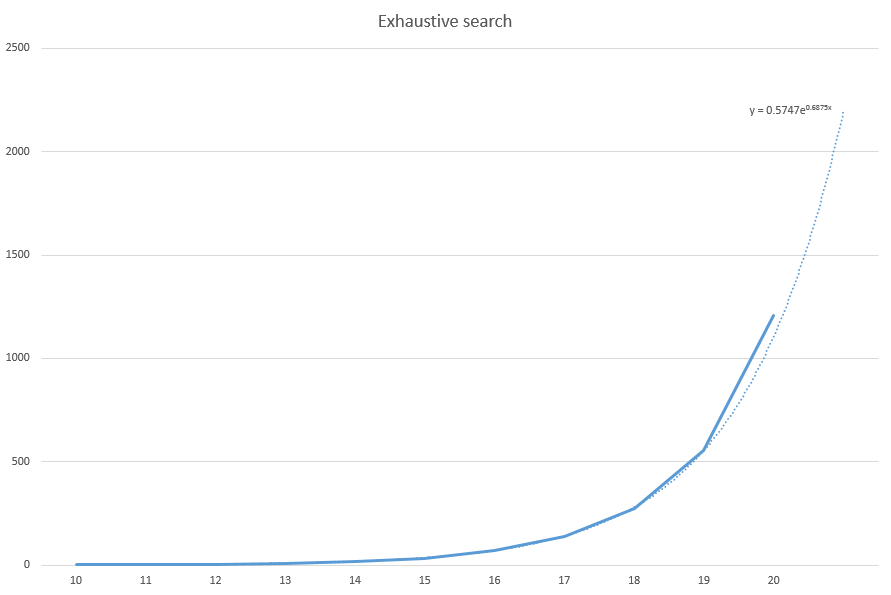
\includegraphics[width=0.7\textwidth]{img/exh2}
\end{center}

Average time in $100\times$ seconds [TODO: REDO EXPERIMENT] for randomly generated instances with $n=\ell$ for $n=10,\ldots,20$.

Dotted line: fitted exponential curve.

\end{frame}

\begin{frame}
{Greedy method}

Find the variable that appears most often and assign it accordingly to maximize ...

%        variables_occurance = [[i,0] for i in range(-self.nv,self.nv+1)] # if i != 0]
%        for c in self.clauses:
%	        for v in c:
%		        variables_occurance[ v+self.nv ][1] += 1
%        variables_occurance.sort( key=lambda a:a[1] ) #, reverse=True )
%        for v in variables_occurance:
%	        self.variable_assignment[ abs(v[0])-1 ] = (v[0]>0)
%        return self.ratio_satisfied()

\begin{algorithmic}[1]\sffamily
	\State $L \gets \emptyset$
	\For{$w\in\{x_1,\lnot x_1,\ldots,x_n,\lnot x_n\}$}
		\State Count occurrences of $w$ in $\phi$
		\State Append pair $(w, \text{count of occurrences of $w$ in $\phi$})$ to $L$
	\EndFor
	\State Sort $L$ with respect to the second component
%	\State\Comment{We now have the literals in decreasing order of total occurrence}
	\For{$(w,c)\in L$}
		\State Set $w$ to True \Comment{If $w=\lnot x_i$ then set $x_i$ to False}
	\EndFor
	\State \Return count of satisfied clauses
\end{algorithmic}

\vfill

Cost: $O(n\log n)$ assuming the use of an $O(n\log n)$ sorting algorithm.
\end{frame}

\begin{frame}
\begin{center}
	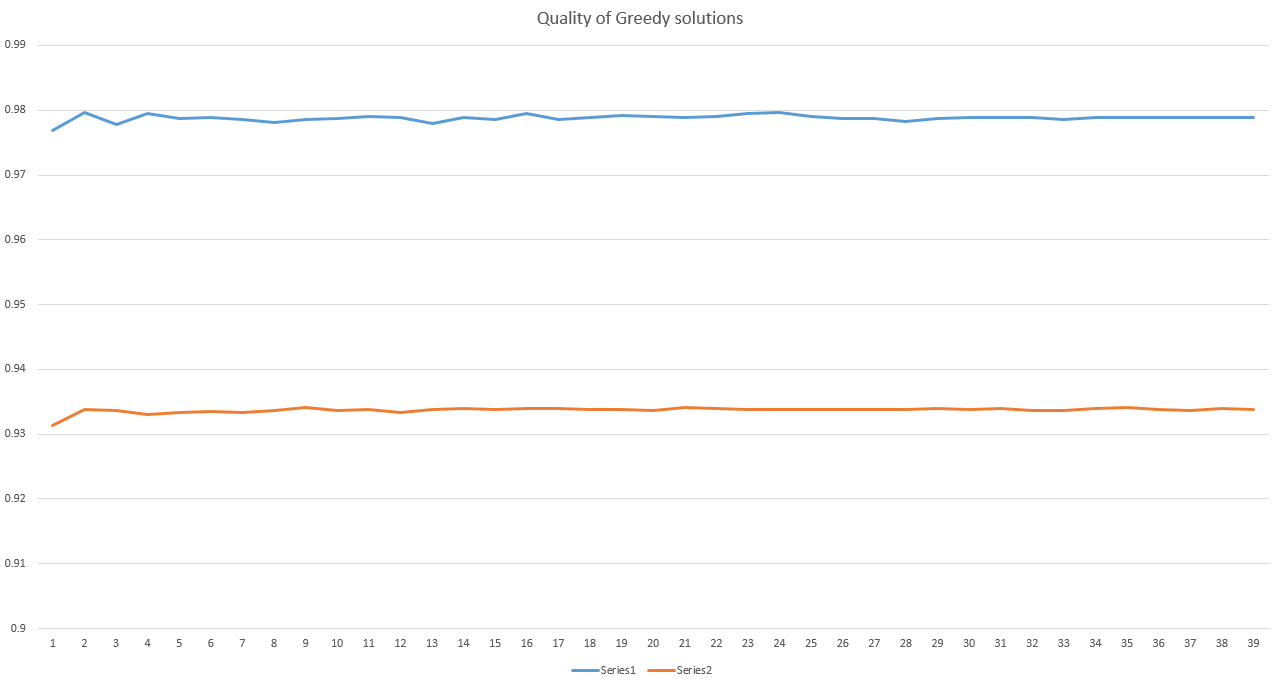
\includegraphics[width=\textwidth]{img/greedy1}
\end{center}

Average ratio of clauses satisfied by Greedy. [TODO: WRONG X-AXIS VALUES]
Blue when $\rho=1$ giving about $98\%$, and orange when $\rho=10$ dropping to about $93\%$.
\end{frame}

%
%
% =======================================================================
%
%

\begin{frame}
{References}
	
	\begin{thebibliography}{References}
		\beamertemplatebookbibitems
		\bibitem{t4}
		Hoos, H. and Stutzler, T. (2005)
		\textbf{Stochastic Local Search: Foundations and Applications.}
		Morgan Kaufmann

		\bibitem{t2}
		Garey, S. and Johnson, D. (1979)
		\textbf{Computers and Intractability: A Guide to the Theory of NP-Completeness.}
		Freeman
				
	\end{thebibliography}
	
\end{frame}

\end{document}